In~\cite{Weghe2007}, the triangular model framework is introduced, based on~\cite{Kulpa1997}. In~\cite{DeTre2012}, the framework is generalized to allow the representation of and reasoning with time intervals subject to uncertainty. In this section, this generalization's main aspects are briefly presented. 

\subsection{\label{subsec:tm-preliminaries}Preliminary Concepts}
Usually, different time intervals are visualized as different parallel line segments in the image plane. However, as this linear approach introduces a few difficulties, the TM framework was conceived to visualize time intervals as points in the image plane.

To achieve this, on the image plane, a horizontal line segment visualizing the used (part of the) time axis is drawn. Then, a triangle is drawn, using this line segment as a side of which the angles with the other two sides have sizes $\alpha$ and $-\alpha$ respectively. The area contained in this triangle is called the \emph{interval space} and will contain all visualizations of intervals. Now, the procedure used to visualize a crisp time interval $\left[s, e\right]$ in the interval space is the following:

\begin{enumerate}
	\item Visualize $s$ as a point on the visualization of the time axis.
	\item Construct a straight half-line $L_s$ from this point, with an angle of size $\alpha$ with the visualization of the time axis.
	\item Visualize $e$ as a point on the visualization of the time axis.
	\item Construct a straight half-line $L_e$ from this point, with an angle of size $-\alpha$ with the visualization of the time axis.
	\item The intersection point of $L_s$ and $L_e$ is the visualization of interval $\left[s, e\right]$.
\end{enumerate}

The resulting point visualizing an interval is generally called an \emph{interval point}. In this work, as it is usually done, the size of $\alpha$ is chosen to be $45^{\circ}$. An example of such construction is shown in figure \ref{fig:tm-const-ex}.

\begin{figure}[h]
	\centering
	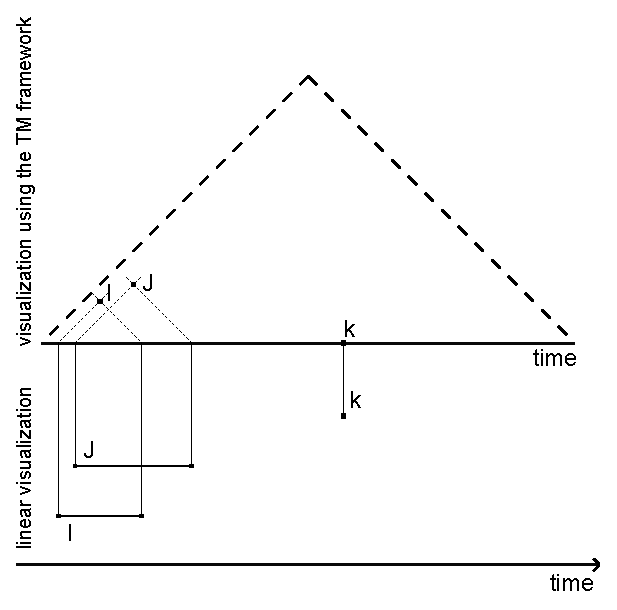
\includegraphics[width=0.8\columnwidth]{graphs/TM_model_several.eps}
	\caption{The visualization of several time intervals using the TM framework.}
	\label{fig:tm-const-ex}
\end{figure}


%Time intervals are usually represented in a one dimensional scale. This is due to its linear characteristic. This approach has also been used in Figure\ref{fig:allen-relationships} and \ref{fig:ill-known-ti}. The difficulty of accurate visual analysis on the temporal data arises when the number of time intervals increase. 

%The triangular model (TM) ~\cite{Kulpa1997}, \cite{Weghe2007} represents time intervals in a two dimensional space called IRterval point completely determines the start and end of the interval. The two-dimensional space of interval points is called the interval space and is denoted by IR ~\cite{Kulpa2006}. The procedure to represent a time interval $[t_s, t_e]$ as an interval point in a two dimensional space is the following:

%\begin{enumerate}
%\item Draw each time point of the interval $[t_s, t_e]$ in the horizontal line.
%\item Construct one straight line $L_s$ from $t_s$ with an angle $\alpha$.
%\item Construct one straight line $L_e$ from $t_e$ with an angle $-\alpha$.
%\item The intersection of these two lines is the interval point.
%\end{enumerate}

%For the shake of simplicity, in this work, the angle for $\alpha$ is chosen to be $45^{\circ}$.

%In TM, these thirteen Allen relations each correspond to a specific zone in the interval space IR \cite{Kulpa1997}. These thirteen zones are called Crisp Relational Zones (CRZs). The CRZs with respect to a reference interval point $I$ are depicted in Figure \ref{fig:allencrz}. 

%\begin{figure}[h]
%   \centering
%   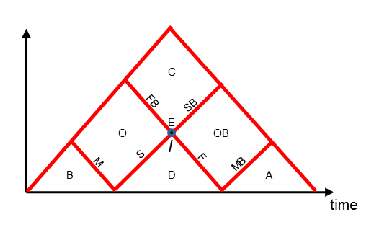
\includegraphics[width=0.8\columnwidth]{graphs/allencrc.eps}
%   \caption{CRZs corresponding to the thirteen Allen's relations. The following shorthand notations are used: equals (E), starts (S), started by (SB), finishes (F), finished by (FB), meets (M), met by (MB), overlaps (O), overlapped by (OB), during (D), contains (C), before (B) and after (A).  }
%   \label{fig:allencrz}
% \end{figure}

%Each CRZ represents the set of interval points of the crisp time intervals that are in the corresponding Allen relation with respect to the reference interval $I$. For example, all interval points of intervals that come before $I$ are located in the CRZ represented by the leftmost lower triangle in the interval space. Likewise, if an interval point is located in the top quadrangle above $I$, then its corresponding interval contains $I$. CRZs allow to visually analyse relations between (large) sets of interval points.

\subsection{\label{subsec:tm-interval}Representation of Uncertainty in Intervals}
The TM framework allows uncertainty in time intervals by supporting uncertain time intervals:

\begin{definition}
Given an ordered set of instants $T$, an \emph{uncertain time interval} (UTI) $J$ in $T$ is here a time interval defined by a pair
\begin{align}
J \triangleq (\pi_s, \pi_e)
\end{align}
where $\pi_s$ and $\pi_e$ are two convex possibility distributions on $T$.
\end{definition}

For a UTI $J$ defined by $(\pi_s, \pi_e)$ with $\pi_s$ and $\pi_e$ two possibility distributions on an ordered set of instants $T$, $\pi_s$ and $\pi_e$ define the confidence that an instant in $T$ is the starting instant, respectively the ending instant of $J$. Because for such UTI $J$, $\pi_s$ and $\pi_e$ are required to be convex, the possibility $\pi_J(I)$ that a given crisp time interval $I = \left[s_i, e_i\right]$ is the exact time interval represented by $J$ can be uniquely determined by:

\begin{align}
\pi_J(I) = \begin{cases}
 \min \left(\pi_s (s_i), \pi_e (e_i) \right), & \mbox{ if } s_i \leq e_i\\
0, & \mbox{ otherwise }
\end{cases}
\end{align}

An UTI $J$ defined by a pair $(\pi_s, \pi_e)$ is now visualized as an area in the image plane, using a single-color greyscale. Every crisp time interval $I$ for which the possibility $\pi_J(I)$ of $I$ being the time interval represented by $J$ is higher than zero, is considered. For every such $I$, the interval point is drawn and is given the greyscale color which reflects the possibility that $I$ is the time interval represented by $J$. For this, a single-color greyscale is used where the saturation of the color is linearly related to the possibility. Thus, every interval point in this visualization corresponds to an interval with a higher-than-zero possibility of being the time interval represented by the UTI. An example of such construction is shown in figure \ref{fig:tm-ill-const-ex}. In this figure, a darker color indicates a higher possibility and a lighter color indicates a lower possibility.

\begin{figure}[h]
	\centering
	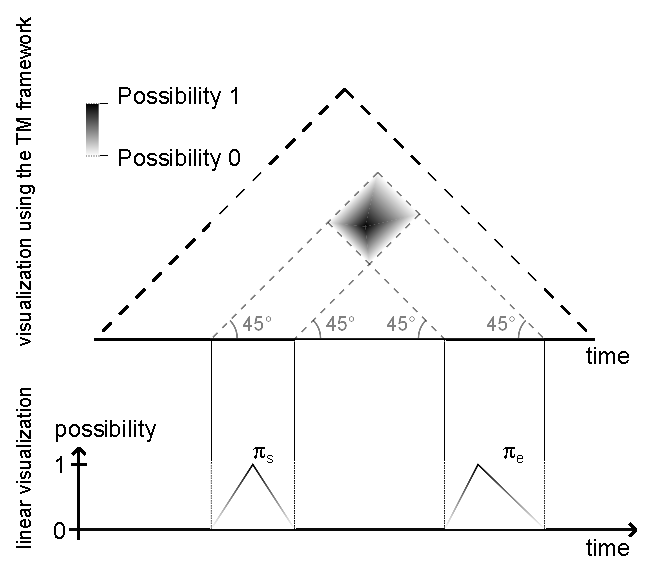
\includegraphics[width=0.8\columnwidth]{graphs/TM_model_ill_known.eps}
	\caption{The visualization of a UTI defined by a pair $(\pi_s, \pi_e)$ using the TM framework.}
	\label{fig:tm-ill-const-ex}
\end{figure}

\subsection{\label{subsec:tm-evaluation}Evaluation of Allen Relationships}
At the base of the evaluation of Allen relationships in the TM framework is the concept of uncertain relational zones.

\begin{definition}
For a given UTI $J$, the \emph{uncertain relational zones} (URZ) are fixed areas in the interval space.
\end{definition}

Now, given an UTI $J$, the procedure to visualize its URZ is the following:


\begin{enumerate}
	\item Determine the visualizations (the points) of both the smallest and greatest instant with a non-zero possibility of being the starting instant of $J$.
	\item Construct two straight half-lines from each of these points: one with an angle of size $\alpha$ with the visualization of the time axis and one with an angle of size $-\alpha$ with the visualization of the time axis. The parts of these half-lines that lie outside of the interval space are not of interest.
	\item Determine the visualizations (the points) of both the smallest and greatest instant with a non-zero possibility of being the ending instant of $J$.
	\item Construct two straight half-lines from each of these points: one with an angle of size $\alpha$ with the visualization of the time axis and one with an angle of size $-\alpha$ with the visualization of the time axis. The parts of these half-lines that lie outside of the interval space are not of interest.
	\item The thusly constructed lines divide the interval space in at most fifteen different areas, including the area corresponding to the visualization of $J$ itself. These areas are $J$'s URZ.
\end{enumerate}

In this procedure, $\alpha$ is the same angle as in the procedure for the visualization of crisp time intervals. The results of this procedure for an example UTI $J$ (as wel as the $J$ itself) are shown in figure \ref{fig:tm-urz}. 

\begin{figure}[h]
	\centering
	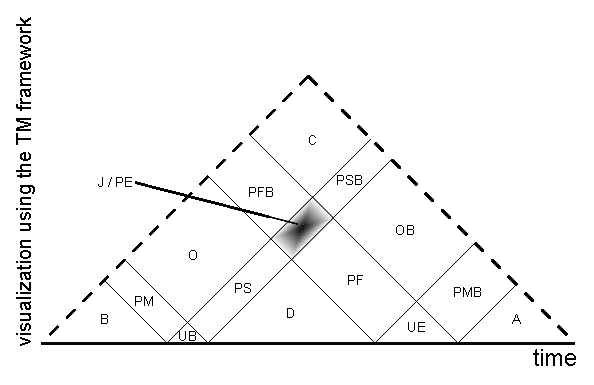
\includegraphics[width=0.8\columnwidth]{graphs/TM_model_URZ.eps}
	\caption{The visualization of the URZ for a given UTI $J$.}
	\label{fig:tm-urz}
\end{figure}

Given a UTI $J$ and its URZ, every URZ is assigned a symbol and a name and corresponds to a set of Allen relationships. The symbol and name are used to uniquely identify each of $J$'s URZ. The set of Allen relationships corresponding to an URZ contains every Allen relationship in which the intervals visualized by the URZ's interval points could be with the interval represented by $J$, depending on what time interval $J$ actually represents. In figure \ref{fig:tm-urz}, the URZ symbols are also shown. In table \ref{tab:urz}, every different row corresponds to a different URZ for a given UTI. In the first two columns, the symbol and name of the URZ are given, the last column contains the set of corresponding Allen relationships. For these, the following notations are used:

\begin{itemize}
	\item `E' denotes `equals'.
	\item `S' denotes `starts'.
	\item `SB' denotes `started by'.
	\item `F' denotes `finishes'.
	\item `FB' denotes `finished by'.
	\item `M' denotes `meets'.
	\item `MB' denotes `met by'.
	\item `O' denotes `overlaps'.
	\item `OB' denotes `overlapped by'.
	\item `D' denotes `during'.
	\item `C' denotes `contains'.
	\item `B' denotes `before'.
	\item `A' denotes `after'.
\end{itemize}

\begin{table}[h]
\centering
\begin{tabular}{|l|l|l|}
\hline
Symbol & Name & Relationships \\
\hline
B    & Before & B \\
O    & Overlaps & O \\
C    & Contains & C \\
D    & During & D \\
OB   & Overlapped by & OB \\
A    & After & A \\
PM   & Possibly meets & M, B, O \\
PS   & Possibly starts & O, S, D \\
PFB  & Possibly finished by & O, FB, C \\
\multirow{2}{*}
{PE}   & Possibly equal  & E, FB, SB, F,\\
       &                 & S, C, D,O, OB \\
PSB  & Possibly started by & C, OB, SB \\
PF   & Possibly finishes & OB, F, D \\
PMB  & Possibly met by & OB, MB A \\
UB   & Uncertain beginning & B, M, O, S, D \\
UE   & Uncertain ending & D, F, OB, MB, A \\
\hline
\end{tabular}
\caption{The fifteen possible URZ for a given UTI.}
\label{tab:urz}
\end{table}

The TM framework now allows evaluating all possible Allen relationships between a given crisp time interval $I$ and a given UTI $J$. This is done as follows. First, $J$ and its URZ are visualized. Next, $I$'s interval point and its construction half-lines $L_s$ and $L_e$ are drawn in the same interval space. Then, evaluation is a matter of positioning (in the following, the possibility that $I$ is in Allen relationship $AR$ with $J$ is denoted  $\Pos(I\ AR\ J)$):

\begin{itemize}
	\item if $I$'s interval point is located in an URZ corresponding with a singleton of Allen relationships $\{R\}$, it is in relationship $R$ with the interval represented by $J$, whichever this interval is. Thus: $\Pos(I\ AR\ J) = 1$.
	\item if $I$'s interval point is located in an URZ corresponding with a non-singleton set of $n$ Allen relationships $\{R_1, R_2, \ldots, R_n\}$, two more half-lines are drawn: one (denoted $L_s'$) from the intersection point of $L_s$ and the visualization of the time axis, its angle with this visualization having size $-\alpha$ and one (denoted $L_e'$) from the intersection point of $L_e$ and the visualization of the time axis, having an angle $\alpha$ with this visualization. Now, some of these half-lines $L_s$, $L_s'$, $L_e$ and $L_e'$ may intersect with the area visualizing $J$. These will divide the area visualizing $J$ in $n$ parts $p_i, 1 \leq i \leq n$ (intersection line segments also count as parts) and each of these parts will correspond to an Allen relationship $R_i$. Now, for each $R_i$:
	\begin{equation}
		\Pos(I\ R_i\ J) = \sup_{I \in p_i} \pi_J(I)
	\end{equation}
\end{itemize}

%TODO: example!

%In this section we will explain a graphical visualization of temporal data called the triangular model (TM). This has been widely used mainly on rough sets for the visualization of historical data. More recently, the model has been extended on possibility theory to model Uncertain Time Intervals (UTI).
%First of all we will explain the main concepts and properties of the triangular model to model Uncertain Time Intervals (UTI). Then, we will detail how to compute the Allen's Relations between a crisp time point and an UTI.

%\subsection{\label{subsec:utis}Uncertain Time Intervals}
%As mentioned in the previous section, the boundaries of time intervals are not always well-known. The available knowledge about the interval can be modelled by using possibility distributions ~\cite{Billiet2012}, ~\cite{JoseEnriquePons2012} on both starting and ending points as mentioned in the previous section. Informally, an Uncertain Time Interval UTI is a time interval for which one or both boundaries are not precisely known. 

%\begin{definition}
% \label{def:uncertain-time-interval}
%An uncertain time interval UTI $I$ is composed by an starting point $S$, and an ending point $E$. For both points, two different convex possibility distributions are defined, namely $\pi_s$, $\pi_e$. These two possibility distributions represent all the possible time intervals that can be constructed from $I$. The following formula obtains the possibility $\pi_{I}$ that a crisp interval  given by  $[a, b]$ is constructed from $I$. 
%\begin{equation}
% \label{eq:possibility-uti}
%\pi_{I} \left(\left[t_s, t_e\right] \right) = 
%\begin{cases}
% \min \left(\pi_s (t_s), \pi_e (t_e) \right), & \mbox{ if } t_s \leq t_e\\
%0, & \mbox{ otherwise. }
%\end{cases}
%\end{equation}

%In the following we will note an UTI as $\pi_{I} = \left(\pi_s, \pi_e \right)$.
% It is important to notice that, the main diference with respect to the ill-known time interval (see Definition \ref{}) is that an UTI only consider as possible starting and ending points 

%\end{definition}

%\subsection{\label{subsec:visualization-tm}Visualization within the triangular model}

%\subsection{\label{subsec:utis-in-tm}Representation of Uncertain Time Intervals}
%In \cite{DeTre2012} a technique to represent UTIs in the triangular model has been presented. Basically, the procedure is an extension of the method to represent crisp time intervals in the triangular space. An UTI $\pi_I = \left(\pi_s, \pi_e \right)$ can be represented in the triangular model by the following procedure, considering that both $\pi_s, \pi_e$ are given by triangular membership functions (see Section \ref{subsec:fuzzy-numbers}).

%\begin{enumerate}
% \item Let $\pi_s = \left[D_s, a_s, b_s\right]$ a triangular membership function.
%\item Let $\pi_e = \left[D_e, a_e, b_e \right]$ a triangular membership function.
%\item Let $t_s^{-} = D_s - a_s$, and $t_s^{+} = D_s + b_s$.
%\item Let $t_e^{-} = D_e -a_e$, and $t_e^{+} = D_e + b_e$.
%\item Construct two straight lines $L_s^{-}, L_s^{-}$ from $t_s^{-}, t_s^{+}$ with an angle $\alpha$.
%\item Construct two straight lines $L_e^{-}, L_e^{-}$ from $t_e^{-}, t_e^{+}$ with an angle $-\alpha$.
%\end{enumerate}

%The intersection of these lines is a quadrangle zone where the UTI is contained. Note that not all the interval points in this zone are to the same extent representing candidate intervals for the UTI.  A grey scaled color gradient is obtained from Eq. \eqref{eq:possibility-uti}. As shown in Fig. \ref{fig:utitm} the color black is associated with a possibility degree of 1, whereas the color white is used when the possibility is 0.
%Equation \eqref{eq:possibility-uti} computes the possibility obtained for the UTI with respect to a candidate interval.
% This formula is used to calculate a grey scaled gradient in which the color black denotes the possibility degree 1 and the color white denotes the possibility degree 0.

%\begin{figure}[h]
%   \centering
%   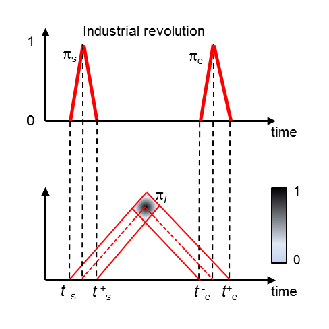
\includegraphics[width=0.8\columnwidth]{graphs/utitm.eps}
%   \caption{Representation in the triangular model for an UTI $\pi_I$.  }
%   \label{fig:utitm}
% \end{figure}

%\subsection{\label{subsec:relational-info-uti}Obtaining Relational Information}
%In order to make temporal reasoning with UTIs, in the triangular model, the thirteen Allen's Relations, and its respective Crisp Relational Zones (CRZ) have been generalized. In this case, we obtain fifteen Uncertain Relational Zones (URZ) , shown in Fig. \ref{fig:urz} and in Table \ref{tab:urz}. 

%\begin{figure}[h]
%   \centering
%   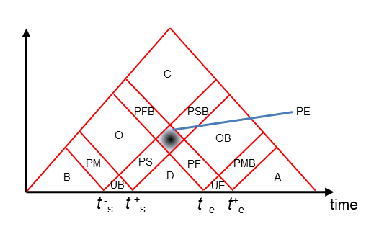
\includegraphics[width=0.8\columnwidth]{graphs/urz.eps}
%   \caption{Uncertain Relational Zones (URZ) for a given UTI.  }
%   \label{fig:urz}
% \end{figure}




%The way to obtain the relational information between an interval point $J = \left[s_j, e_j \right]$, and an UTI $\pi_I$ depends on the location of $J$ with respect to the UTI $\pi_I$:

%\begin{itemize}
% \item If $J$ is located in a zone with only one possible Allen relation, then it is true that $J$ is in the relation. (And therefore, the possibility is always 1).
%\begin{equation}
% \label{eq:possibility-iz-uti-certain}
%\mu_{\left(J R \pi_I \right)} \left(R \right) = 1.
%\end{equation}


%\item If $J$ is located in a zone with multiple candidate Allen's relations, then there is uncertainty about the Allen relation that applies between $J$ and the UTI $\pi_I$. The procedure to obtain the possibility degree is the following:

%\begin{enumerate}
% \item Draw the lines $L_s, L_e$ that represent the interval point $J$, with the procedure shown in Section \ref{subsec:visualization-tm}. 
%\item Draw the orthogonal lines from $L_s, L_e$. 
%\item One or several of these lines could intersect with the UIZ of $\pi_I$. Then, the UIZ is divided into as many different subzones $\pi_I^{R'}$ as possible candidate Allen relations $R'$ between $J$ and $\pi_I$ exist.
%\item $\pi_I^{R'}$ is the zone that correspond to a candidate Allen Relation $R'$.
%\end{enumerate}
%The possibility that a candidate relation $R'$ is the actual relation between $J$ and $\pi_I$ is given by:
%\begin{equation}
% \label{eq:possibility-iz-uti}
%\mu_{\left(J R \pi_I \right)} \left(R' \right) = \sup_{I \in \pi_I^{R'}} \pi_I(I).
%\end{equation}
%\end{itemize}

%\begin{figure}[h]
%   \centering
%   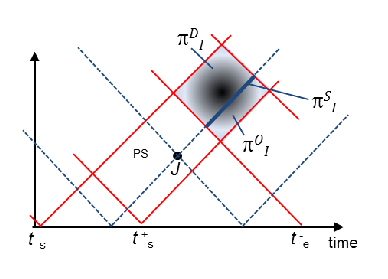
\includegraphics[width=0.8\columnwidth]{graphs/calculation.eps}
%   \caption{Uncertain Relational Zones (URZ) for a given UTI.  }
%   \label{fig:calculation}
% \end{figure}

% Mainly due to its linear characteristic, time is traditionally visualised using a linear representation where several time intervals are depicted as linear segments on top of a horizontal time axis. This approach has also been used in Fig. \ref{fig:ill-known-ti}. One can read the start and end point of each interval the horizontal scale. The vertical dimension is solely used to differentiate multiple overlapping intervals, if used at all. The linear representation works well as long as the number of represented time intervals remains low. As soon as a large number of overlapping intervals have to be represented the representation becomes overloaded and accurate visual data analysis becomes almost impossible.


% For that reason, an alternative Triangular time Model (TM) has been presented in \cite{Weghe2007}. This model is an extension of Kulpa's triangular model for the modelling of crisp time intervals \cite{Kulpa1997}. Basically, intervals are modelled as interval points in a two-dimensional space as follows. First, a horizontal time axis is considered. Second, for each time interval $\left[t_s, t_e \right]$ two straight lines $L_s$ and $L_e$ are constructed as depicted in Fig. \ref{}. Line $L_s$ is passing through $t_s$ and makes a fixed angle $\alpha$ with the horizontal time axis, whereas Le is passing through te making a fixed angle $-\alpha$ with the horizontal time axis. The interval $\left[t_s, t_e \right]$ is then represented by the intersection of $L_s$ and $L_e$ , which is called the interval point of $\left[t_s, t_e \right]$. For the ease of use, $\alpha$ is here chosen to be $45^{\circ}$ . In TM all time intervals are represented by their corresponding interval point. So, because $\alpha$ is fixed for all interval points, the position of the interval point completely determines the start and end of the interval. The two-dimensional space of interval points is called the interval space and is denoted by IR \cite{Kulpa2006}.

%Figure 3

% From the observation that the start points and end points of two crisp time intervals $I^{1} = \left[t_s^1, t_e^1 \right]$ and $I^2 = \left[t_s^2, t_e^2 \right]$ can be smaller than ($<$), equal to ($=$) or larger than ($>$) each other, Allen proposed the thirteen possible relations between two crisp time intervals given in Table \ref{} \cite{Allen1983}.
% 







% \subsection{\label{subsec:uncertainty-about-time-intervals}Uncertainty about Time Intervals}
% Time is a complex natural phenomenon that, among others, allows humans to organise life and plan activities. Time also plays an important role in information management as it allows to register facts with different kinds of timestamps and make use of these timestamps during querying and information retrieval. Dealing with time in an information system requires a time model. In this paper, it is implicitly assumed that time is modelled as being discrete, linear and finite. This means that it is considered that time can only be/ observed using a limited precision, say $\delta$. Observing time using a maximum precision $\delta$ and with respect to a given origin $t_0$ involves a crisp discrete (countable) set of time points, given by
% \begin{equation}
%  \label{eq:t0-delta}
% T_{0,\delta} = \lbrace t_K \in T | t_k = t_0 + k\delta, k \in \Z \rbrace
% \end{equation}
% 
% where $Z = \left \lbrace 0, 1, -1, 2, -2, \ldots \rbrace \right. T_{0, \delta}$ is a proper subset of the continuum $T$ of the physical time points. The discretisation can be described as a surjective mapping from $T$ on $T_{0,\delta}$, which maps each $\tau \in T$ on the element $t_k \in T_{0,\delta}$ that lies in the interval
% \begin{equation}
% \gamma_{0,k} = \left[ t_0 + k\delta, t_0 + (k+1)\delta \right[, k \in \Z 
% \end{equation}
% 
% Discretisation implies that all time points within an interval $\gamma_{0,k}$ are considered to be indistinguishable and mapped to the same time point $t_k$. This is not really a limitation, on condition that the precision $\delta$ is chosen sufficiently accurate. The discretisation is necessary to circumvent the density problem (i.e., the fact that between any two distinct points, there always exists at least one other point). Linearity implies a total order over the time points. Finally, our model is chosen to be finite in view of a computer representation. This implies that all values that exceed the determined upper and lower bound will be handled by introducing two special values $(- \infty $ and  $+\infty)$.
% 
% The intervals $\gamma_{0,k}$ with $\delta$ as length are usually called `chronons' in literature (cf. \cite{Dyreson1994}). The introduction of chronons eliminates the necessity of making a distinction between points and intervals, because even a chronon, the smallest unit in the model, is essentially an interval. 
% 
% A time interval $\left[t_s, t_e \right]$ is defined by a start time point $t_s$  and a length $l$, which defines the distance (number of chronons) from ts to the end time point $t_e$, i.e., $l = t_e - t_s$.
% 
% 
% A time point is equivalent to a time interval with $l = 0$ (or $t_e = t_s$ ). Note that the length of an interval is not the same as the duration of the interval: the length of a time point is 0, its duration is 1 chronon ($\delta$). 
% 
% In practice, it often occurs that time intervals cannot be exactly specified. Especially, in historical data it is often the case that either the starting date or the ending date (or both) of a time interval are partially or completely unknown. In such cases, the best thing to do is modelling the available knowledge about (the uncertainty of) the interval as accurate as possible, hereby avoiding information loss. Soft computing techniques, more specifically possibility theory \cite{DidierDubois1988a}, can be used for that purpose. In \cite{Billiet2012}, \cite{JoseEnriquePons2012} a possibilistic valid time model able to cope with time intervals that have an uncertain start and/or end point has been presented. The basics of this model are used in this paper and briefly described as follows. Each (Un)certain Time Interval (UTI) is defined by a pair
% \begin{equation}
%  \label{eq:uncertain-time-interval}
% \left(\pi_s, \pi_e \right)
% \end{equation}
% 
% where $\pi_s$ and $\pi_e$ are two convex possibility distributions, respectively reflecting the knowledge about the start and end point of the UTI (as illustrated in Fig. \ref{}(a)). In case of certainty, the possibility distribution is characterised by a fuzzy set with singleton support and core containing the crisp date. In case of uncertainty, the possibility distribution is characterised by a fuzzy set containing all possible candidate values for the date and their associated degree of possibility. 
% % figura 2
% 
% Together, both possibility distributions reflect the available knowledge about the start and end of the UTI they model. This implies that $\pi$s and $\pi$e together represent another possibility distribution $\pi$I consisting of all possible time intervals that can be constructed from $\pi$s and $\pi$e . Some of the intervals in $\pi_I$ are depicted in Fig. \ref{}(b). For each time interval $\left[t_s , t_e \right]$, its associated possibility grade in $\pi_I$ is computed by
% \begin{equation}
%  \label{eq:possibility-uti}
% \pi_{I} \left(\left[t_s, t_e\right] \right) = 
% \begin{cases}
%  \min \left(\pi_s (t_s), \pi_e (t_e) \right), & \mbox{ if } t_s \leq t_e\\
% 0, & \mbox{ otherwise. }
% \end{cases}
% \end{equation}
% 
% Eq. \eqref{eq:possibility-uti} reflects that given the uncertainty about the start point, modelled by $\pi$s and the uncertainty about the end point, modelled by $\pi_e$ $\pi$e , the possibility that $\left[t_s, t_e \right]$ is the actual value of the UTI equals the possibility that ts is the actual start point (i.e., $\pi_s (t_s)$) and te is the actual end point (i.e., $\pi_e (t_e)$) of $I$, where the conjunction of both conditions is modelled by the minimum t-norm. In the inconsistent case where $t_s > t_e$ the interval is considered to be completely impossible. In the remainder of this paper we will denote an UTI as $\pi_I$, i.e., $\pi_I = \left( \pi_s, \pi_e \right)$.


% 
% \subsection{\label{subsec:the-triangular-model}The triangular model}
% Mainly due to its linear characteristic, time is traditionally visualised using a linear representation where several time intervals are depicted as linear segments on top of a horizontal time axis. This approach has also been used in Fig. \ref{}(b). One can read the start and end point of each interval the horizontal scale. The vertical dimension is solely used to differentiate multiple overlapping intervals, if used at all. The linear representation works well as long as the number of represented time intervals remains low. As soon as a large number of overlapping intervals have to be represented the representation becomes overloaded and accurate visual data analysis becomes almost impossible.
% 
% For that reason, an alternative Triangular time Model (TM) has been presented in \cite{Weghe2007}. This model is an extension of Kulpa's triangular model for the modelling of crisp time intervals \cite{Kulpa1997}. Basically, intervals are modelled as interval points in a two-dimensional space as follows. First, a horizontal time axis is considered. Second, for each time interval $\left[t_s, t_e \right]$ two straight lines $L_s$ and $L_e$ are constructed as depicted in Fig. \ref{}. Line $L_s$ is passing through $t_s$ and makes a fixed angle $\alpha$ with the horizontal time axis, whereas Le is passing through te making a fixed angle $-\alpha$ with the horizontal time axis. The interval $\left[t_s, t_e \right]$ is then represented by the intersection of $L_s$ and $L_e$ , which is called the interval point of $\left[t_s, t_e \right]$. For the ease of use, $\alpha$ is here chosen to be $45^{\circ}$ . In TM all time intervals are represented by their corresponding interval point. So, because $\alpha$ is fixed for all interval points, the position of the interval point completely determines the start and end of the interval. The two-dimensional space of interval points is called the interval space and is denoted by IR \cite{Kulpa2006}.
% 
% %Figure 3
% 
% From the observation that the start points and end points of two crisp time intervals $I^{1} = \left[t_s^1, t_e^1 \right]$ and $I^2 = \left[t_s^2, t_e^2 \right]$ can be smaller than ($<$), equal to ($=$) or larger than ($>$) each other, Allen proposed the thirteen possible relations between two crisp time intervals given in Table \ref{} \cite{Allen1983}.
% 
% In TM, these thirteen Allen relations each correspond to a specific zone in the interval space IR \cite{Kulpa1997}. These thirteen zones are called Crisp Relational Zones (CRZs). The CRZs with respect to a reference interval point $I$ are depicted in Fig. \ref{}. Hereby, the following shorthand notations are used: equals (E), starts (S), started by (SB), finishes (F ), finished by (F B), meets (M ), met by (M B), overlaps (O), overlapped by (OB), during (D), contains (C), before (B) and after (A).
% 
% % TABLE I
% % T HE THIRTEEN POSSIBLE A LLEN RELATIONS BETWEEN CRISP TIME
% % INTERVALS
% % 
% % I 1 equals I 2
% % I 1 starts I 2
% % I 1 started by I 2
% % I 1 f inishes I 2
% % I 1 f inished by I 2
% % I 1 meets I 2
% % I 1 met by I 2
% % I 1 overlaps I 2
% % I 1 overlapped by I 2
% % I 1 during I 2
% % I 1 contains I 2
% % I 1 bef ore I 2
% % I 1 af ter I 2
% 
% Each CRZ represents the set of interval points of the crisp time intervals that are in the corresponding Allen relation with respect to the reference interval $I$. For example, all interval points of intervals that come before $I$ are located in the CRZ represented by the leftmost lower triangle in the interval space. Likewise, if an interval point is located in the top quadrangle above $I$, then its corresponding interval contains $I$. CRZs allow to visually analyse relations between (large) sets of interval points.